% main.tex - A Mathematical Model of Contextual Capabilities
\documentclass[11pt,a4paper]{article}

% Page geometry
\usepackage[margin=1in]{geometry}

% Custom macros
\usepackage{main}

% Additional packages
\usepackage{booktabs}
\usepackage{graphicx}
\usepackage{subcaption}
\usepackage{enumitem}
\usepackage{microtype}

% Hyperref configuration
\hypersetup{
  colorlinks=true,
  linkcolor=blue!70!black,
  citecolor=green!50!black,
  urlcolor=blue!70!black,
  pdftitle={A Mathematical Model of Contextual Capabilities},
  pdfauthor={Fengyun Liu, TypeScope; Ondrej Lhotak, University of Waterloo},
  pdfsubject={Capability-based security, formal verification},
  pdfkeywords={capabilities, security, formal methods, Coq, lambda calculus}
}

\pdfstringdefDisableCommands{%
  \def\lambdaCC{lambda-CC}%
  \def\lambdaCap{lambda-CC}%
}

% Title information
\title{\textbf{A Mathematical Model of Contextual Capabilities}\\[0.5em]
\large Formally Verified Static Capability Tracking in
\texorpdfstring{\lambdaCC}{lambda-CC}}

\author{Fengyun Liu\\TypeScope \and Ond\v{r}ej Lhot\'ak\\University of Waterloo}
\date{}

\begin{document}

\maketitle

\begin{abstract}
  Capability-based security offers a principled way to enforce least privilege,
  but three gaps remain. %
  Traditional capability systems such as the object-capability model typically
  do not support static checking of capability usage. %
  Meanwhile, manual propagation of capabilities through every interface incurs
  substantial boilerplate when multiple fine-grained capabilities are
  involved. %
  Finally, existing capability systems do not always treat capabilities as
  abstract interfaces to enable simulation and testing. %

  We present \lambdaCC{}, a minimal calculus of \emph{contextual capabilities}:
  capabilities that are both statically tracked and selectively supplied by the
  surrounding calling context. %
  The development is mechanized in Coq. %
  Although \lambdaCC{} is intentionally minimal, it provides a mathematical core
  for designing secure programming languages with statically checked capability
  propagation, authority attenuation, and safe execution of untrusted code. %
\end{abstract}

\vspace{1em}
\noindent\textbf{Keywords:} capability-based security, formal verification,
capability systems, lambda calculus

\tableofcontents

\newpage

% Include all sections
% introduction.tex - Introduction to the Lambda^Cap white paper

\section{Introduction}
\label{sec:introduction}

Software systems increasingly execute code that is neither fully trusted nor
fully reviewed before deployment. %
Some of this code comes from plugins or user-defined scripts. %
Increasingly, it is generated on demand by large language models. %
In all of these settings, the security problem is the same: how do we ensure
that code receives exactly the authority it needs, and no more?

This is a \emph{least-privilege} problem: authority should be explicit, bounded,
and reviewable rather than ambient \cite{saltzer-schroeder}. %
Capability-based security gives the right general answer to least privilege and
confused-deputy problems \cite{hardy-confused}, %
but past capability models and capability-oriented languages such as E and Joe-E
leave several important problems unresolved \cite{e-lang,joe-e}. %

This paper presents a mechanized mathematical model of \emph{contextual
  capabilities}. %
The main purpose of the model is to provide a foundation for designing new
secure programming languages in which authority is explicit, statically tracked,
and controlled by program context. %

\subsection{Research Gap}

There are three major limitations in past capability models that affect the
usability of secure programming languages. %

First, a capability system should support \emph{static checking of capability
  usage}. %
It should be possible to read a function's type signature as a trustworthy upper
bound on the capabilities it may use. %
The object-capability model \cite{miller-robust,miller-paradigm} gives a strong
design discipline, %
but it does not by itself provide a compact type-level account of capability use
that can be checked compositionally. %

Second, a capability system should facilitate the \emph{propagation of
  fine-grained capabilities}. %
Capability-based programs do not carry a single coarse permission; they pass
user-scoped services, output channels, loggers, tool bindings, and other narrow
capabilities through higher-order code. %
Without language support, manual propagation through every interface quickly
becomes boilerplate-heavy. %
A useful model should make such propagation explicit and compositional, without
collapsing these capabilities into ambient authority. %

Third, a capability system should support \emph{simulation and testing} by
treating capabilities as abstract interfaces rather than hidden ambient
mechanisms. %
When capabilities remain explicit program values, the same program structure can
be exercised against restricted, attenuated, or mocked capabilities. %
Existing capability systems do not always make that form of substitution natural
at the level of the model. %

\subsection{Contextual Capabilities}

This paper proposes a mathematical model of \emph{contextual capabilities}. %
The basic idea is that capabilities are ordinary typed values that can be
explicitly provided or rebound for a context. %
Code deep in a call chain may then use them without every intermediate function
carrying them as ordinary parameters. %
Their use is tracked statically, but their availability is determined by
surrounding program context rather than by ambient authority. %

\subsection{Contribution}

We present \lambdaCC{}, a minimal calculus of contextual capabilities. %
Its contribution is to combine explicit capability values, static capability
tracking, and a higher-order operational account in one verified formalism. %
The resulting model supports reasoning about restricted execution,
capability-sensitive interfaces, authority attenuation, and the safe execution
of untrusted code. %
It is intended as a design model for new secure programming languages, rather
than as a complete implementation strategy by itself. %

% background.tex - Contextual capabilities

\section{Contextual Capabilities}
\label{sec:background}

The easiest way to understand contextual capabilities is to start from a
mechanism every reader already knows: ordinary function parameters. %
If an operation needs an output channel, a logger, and a user-scoped orders
service, one direct design is to pass all of them explicitly:
\[
\texttt{handle(req, out, logger, orders)}
\]
and then continue threading those same parameters through helpers that may not
use them directly:
\[
\begin{array}{l}
\texttt{handle(req, out, logger, orders)} \\
\rightarrow\ \texttt{plan(task, out, logger, orders)} \\
\rightarrow\ \texttt{respond(plan, out, logger, orders)}
\end{array}
\]
This style is explicit and testable, but it is also noisy. %
Intermediate functions often carry capabilities only so later code can
eventually use them. %

Contextual capabilities keep the good part of parameter passing and remove that
plumbing cost. %
A capability is still an ordinary typed value, but it may be \emph{bound for a
  context} rather than passed through every signature. %
Code deeper in the call chain can then use that capability because the
surrounding context makes it available. %
In that sense, capabilities behave like remotely bound parameters that propagate
through the call chain automatically, while remaining statically tracked and
explicitly controllable. %

\begin{figure}[t]
\centering
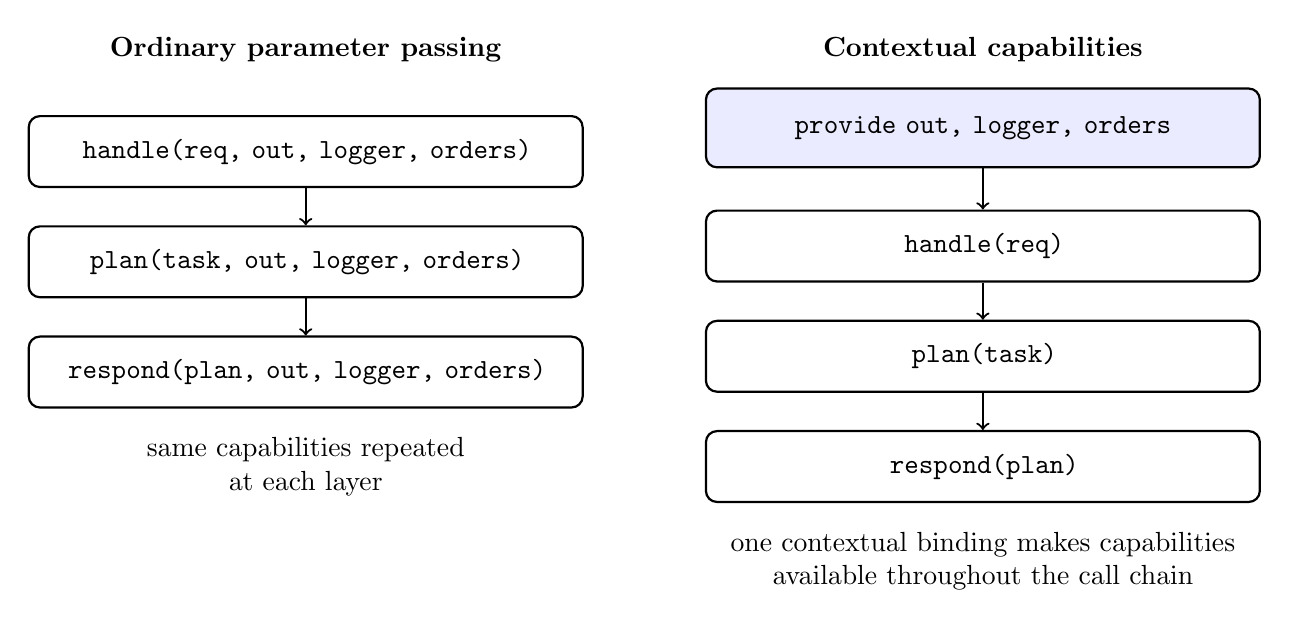
\begin{tikzpicture}[
  fn/.style={draw, rounded corners, thick, align=center, text width=6.8cm, minimum height=0.9cm},
  ctx/.style={draw, rounded corners, fill=blue!8, thick, align=center, text width=6.8cm, minimum height=1.0cm},
  note/.style={align=center}
]
  \node[note] at (-4.3,2.2) {\textbf{Ordinary parameter passing}};
  \node[fn] (h1) at (-4.3,0.9) {\texttt{handle(req, out, logger, orders)}};
  \node[fn] (p1) at (-4.3,-0.5) {\texttt{plan(task, out, logger, orders)}};
  \node[fn] (r1) at (-4.3,-1.9) {\texttt{respond(plan, out, logger, orders)}};
  \draw[->, thick] (h1) -- (p1);
  \draw[->, thick] (p1) -- (r1);
  \node[note] at (-4.3,-3.1) {same capabilities repeated\\at each layer};

  \node[note] at (4.3,2.2) {\textbf{Contextual capabilities}};
  \node[ctx] (c) at (4.3,1.2) {\texttt{provide out, logger, orders}};
  \node[fn] (h2) at (4.3,-0.3) {\texttt{handle(req)}};
  \node[fn] (p2) at (4.3,-1.7) {\texttt{plan(task)}};
  \node[fn] (r2) at (4.3,-3.1) {\texttt{respond(plan)}};
  \draw[->, thick] (c) -- (h2);
  \draw[->, thick] (h2) -- (p2);
  \draw[->, thick] (p2) -- (r2);
  \node[note] at (4.3,-4.3) {one contextual binding makes capabilities\\available throughout the call chain};
\end{tikzpicture}
\caption{Ordinary parameter plumbing versus contextual capability propagation}
\label{fig:contextual-propagation}
\end{figure}

\autoref{fig:contextual-propagation} is the central intuition. %
Contextual capabilities do not make authority ambient. %
They make authority available through explicit program context. %
A caller may bind an output capability for a single execution. %
Trusted code may rebind a user-scoped orders capability for one region of
computation. %
A closure may package a capability behind a narrower interface. %
In each case, the capability remains an ordinary value; what changes is only how
it becomes available to the code that uses it. %

\paragraph{The Challenge.}
The challenge is to give this convenience a sound static account. %
A capability should be usable only when some program context has explicitly
provided it, even in the presence of deep and complex transitive call chains and
first-class functions. %

Lambdas make that harder. %
A closure may carry capability usage transitively: it may use a capability
itself, or call another function that uses it. %
A formal model therefore has to track not only direct capability access, but
also capability use delayed through closure capture and later invocation. %

The calculus \lambdaCC{} provides a formal foundation for statically checked
contextual capabilities. %

% calculus.tex - The Lambda^Cap Calculus

\section{The \lambdaCap{} Calculus}
\label{sec:calculus}

\lambdaCap{} is a small extension of the simply-typed lambda calculus with three
capability constructs: %
capability access $\tmcvar{c}$, %
capability binding $\tmwith{c}{e_1}{e_2}$, %
and capability restriction $\tmallow{\varphi}{e}$. %

We assume the reader is already comfortable with standard formal-language
notions such as syntax, typing judgments, and big-step evaluation for the
simply-typed lambda calculus; Pierce's \emph{Types and Programming Languages} is
a standard reference \cite{pierce-tapl}. %

\autoref{fig:syntax} gives the reader-facing surface syntax. %
Function syntax uses brace notation, while function types place the designated
capability set above the arrow: $\tmabs{x}{T_1}{\varphi}{\varphi}{t}$ denotes a
function that receives the call-site capabilities in $\varphi$, and
$\tarr{T_1}{T_2}{\varphi}{\varphi}$ is the corresponding function type. %
The types of the capabilities named in $\varphi$ are defined in the global
capability declaration $\cpdecl$. %

\begin{figure}[t]
\centering
\begin{align*}
\text{Names} \quad & n \in \mathbb{N} \\[0.25em]
\text{Capability names} \quad & c, d \\[0.25em]
\text{Capabilities} \quad & \varphi ::= \effempty \mid \eff{c} \mid \varphi_1 \effunion \varphi_2 \\[0.25em]
\text{Types} \quad & T ::= \tnat \mid \tarr{T_1}{T_2}{\varphi}{\varphi} \\[0.25em]
\text{Terms} \quad & t ::= \tmconst{n} \mid x \mid \tmcvar{c} \mid
    \tmabs{x}{T_1}{\varphi}{\varphi}{t} \mid \tmapp{t_1}{t_2} \\
    & \quad\;\;\mid \tmwith{c}{e_1}{e_2} \mid \tmallow{\varphi}{e}
    \\[0.25em]
\text{Values} \quad & v ::= \vlconst{n} \mid
    \vlclosshort{x}{t}{\vlenv}{\cpenv}
\end{align*}
\caption{Syntax of \lambdaCap{}}
\label{fig:syntax}
\end{figure}

\subsection{Semantics}
\label{sec:semantics}

Evaluation uses a value environment $\vlenv$ for term variables and a capability
environment $\cpenv$ for capabilities. %
The evaluation judgment
\[
\eval{t}{\vlenv}{\cpenv}{v}
\]
means that $t$ evaluates to $v$ under those environments. %

The rules are shown in \autoref{fig:eval-rules}. %
Capability lookup reads from $\cpenv$. %
Capability binding evaluates a body under an updated capability environment. %
Restriction runs a term in a restricted capability environment. %
The main rule is closure creation: evaluating
$\tmabs{x}{T}{\varphi}{\varphi}{t}$ stores $\cpdiff{\cpenv}{\varphi}$, not the
full capability environment. %

\begin{figure}[t]
\centering
\begin{mathpar}
\inferrule*[Right=\rn{E-Const}]
  { }
  {\eval{\tmconst{n}}{\vlenv}{\cpenv}{\vlconst{n}}}

\inferrule*[Right=\rn{E-Var}]
  {\vlenv(x) = v}
  {\eval{x}{\vlenv}{\cpenv}{v}}

\inferrule*[Right=\rn{E-CVar}]
  {\cplookup{\cpenv}{c} = v}
  {\eval{\tmcvar{c}}{\vlenv}{\cpenv}{v}}

\inferrule*[Right=\rn{E-Abs}]
  { }
  {\eval{\tmabs{x}{T}{\varphi}{\varphi}{t}}{\vlenv}{\cpenv}
        {\langle\tmabs{x}{T}{\varphi}{\varphi}{t},\; \vlenv,\; \cpdiff{\cpenv}{\varphi}\rangle}}

\inferrule*[Right=\rn{E-App}]
  {\eval{t_1}{\vlenv}{\cpenv}{\langle\tmabs{x}{T}{\varphi}{\varphi}{t},\; \vlenv_1,\; \cpenv_1\rangle} \\
   \eval{t_2}{\vlenv}{\cpenv}{v_2} \\
   \eval{t}{(\vlenv_1, x \mapsto v_2)}{(\cpmerge{\cpenv}{\cpenv_1})}{v_3}}
  {\eval{\tmapp{t_1}{t_2}}{\vlenv}{\cpenv}{v_3}}

\inferrule*[Right=\rn{E-With}]
  {\eval{e_1}{\vlenv}{\cpenv}{v_1} \\
   \eval{e_2}{\vlenv}{\cpupdate{\cpenv}{c}{v_1}}{v_2}}
  {\eval{\tmwith{c}{e_1}{e_2}}{\vlenv}{\cpenv}{v_2}}

\inferrule*[Right=\rn{E-Allow}]
  {\eval{e}{\vlenv}{\cprestrict{\cpenv}{\varphi}}{v}}
  {\eval{\tmallow{\varphi}{e}}{\vlenv}{\cpenv}{v}}
\end{mathpar}
\caption{Evaluation rules for \lambdaCap{}}
\label{fig:eval-rules}
\end{figure}

This distinction corresponds to two different use cases. %
Some capabilities are meant to come from the function's creation context and
therefore should be captured in the closure. %
Others are meant to come from the call site and therefore should be supplied by
the caller at invocation time. %

% typing.tex - Type System and Capability Tracking

\subsection{Type System and Capability Tracking}
\label{sec:typing}

\autoref{fig:typing-rules} presents the full system. %
The type system assigns each term both a type and a capability set. %
The type
describes the value produced; the capability set is a static upper bound on
the authority the term may use. %
The judgment
\[
\typ{\cpdecl}{\tpenv}{t}{T}{\varphi}
\]
means that term $t$ has type $T$ and may access capabilities in $\varphi$. %

\begin{figure}[t]
\centering
\begin{mathpar}
\inferrule*[Right=\rn{T-Const}]
  { }
  {\typ{\cpdecl}{\tpenv}{\tmconst{n}}{\tnat}{\effempty}}

\inferrule*[Right=\rn{T-Var}]
  {\tpenv(x) = T}
  {\typ{\cpdecl}{\tpenv}{x}{T}{\effempty}}

\inferrule*[Right=\rn{T-CVar}]
  {c \in \cpdecl \\
   \cpdecl(c) = T}
  {\typ{\cpdecl}{\tpenv}{\tmcvar{c}}{T}{\eff{c}}}

\\

\inferrule*[Right=\rn{T-Abs}]
  {\typ{\cpdecl}{\tpenv, x{:}T_1}{t}{T_2}{\varphi'}}
  {\typ{\cpdecl}{\tpenv}{\tmabs{x}{T_1}{\varphi}{\varphi}{t}}
       {\tarr{T_1}{T_2}{\varphi}{\varphi}}{\varphi' \effdiff \varphi}}


\inferrule*[Right=\rn{T-App}]
  {\typ{\cpdecl}{\tpenv}{t_1}{\tarr{T_1}{T_2}{\varphi}{\varphi}}{\varphi_1} \\
   \typ{\cpdecl}{\tpenv}{t_2}{T_1}{\varphi_2}}
  {\typ{\cpdecl}{\tpenv}{\tmapp{t_1}{t_2}}{T_2}
       {\varphi \effunion \varphi_1 \effunion \varphi_2}}

\inferrule*[Right=\rn{T-With}]
  {\cpdecl(c) = T_1 \\
   \typ{\cpdecl}{\tpenv}{e_1}{T_1}{\varphi_1} \\
   \typ{\cpdecl}{\tpenv}{e_2}{T_2}{\varphi_2}}
  {\typ{\cpdecl}{\tpenv}{\tmwith{c}{e_1}{e_2}}{T_2}
       {\varphi_1 \effunion (\varphi_2 \effdiff \eff{c})}}
\\

\inferrule*[Right=\rn{T-Allow}]
  {\typ{\cpdecl}{\tpenv}{e}{T}{\varphi'} \\
   \varphi' \effsubset \varphi}
  {\typ{\cpdecl}{\tpenv}{\tmallow{\varphi}{e}}{T}{\varphi'}}

\inferrule*[Right=\rn{T-Sub}]
  {\typ{\cpdecl}{\tpenv}{t}{T}{\varphi} \\
   c \in \cpdecl}
  {\typ{\cpdecl}{\tpenv}{t}{T}{\varphi \effunion \eff{c}}}
\end{mathpar}
\caption{Typing rules for \lambdaCap{}}
\label{fig:typing-rules}
\end{figure}

\rn{T-CVar} is the rule that actually uses a capability: accessing $\tmcvar{c}$
adds exactly $c$ to the term's capabilities. %
\rn{T-Abs} is the central rule. %
If the function body may use capabilities $\varphi'$, and the lambda marks
$\varphi$ as caller-provided, then the lambda expression itself requires only
$\varphi' \effdiff \varphi$ at its definition site. %
In other words, capabilities listed in $\varphi$ are expected from the call site
rather than from closure creation. %
The function type records the caller-provided capability set $\varphi$ above the
arrow. %

\rn{T-App} restores caller responsibility: applying a function of type
$\tarr{T_1}{T_2}{\varphi}{\varphi}$ contributes $\varphi$ to the application's
capabilities. %
This is the static counterpart of the runtime semantics, where the closure does
not capture the capabilities in $\varphi$ and the caller must supply them at
application time. %

\rn{T-With} binds a value to capability $c$ and masks that requirement in the
body, so uses of $c$ inside $e_2$ do not remain obligations of the outer
context. %
\rn{T-Allow} turns dynamic restriction into a static contract: if $e$ checks
with capability set $\varphi'$ and $\varphi' \subseteq \varphi$, then
restricting execution to $\varphi$ cannot remove a capability that the term
needs. %
\rn{T-Sub} is standard weakening. %


\subsection{Security Properties}
\label{sec:security}

At a high level, \lambdaCap{} guarantees that
\begin{itemize}[nosep]
\item capability annotations are trustworthy upper bounds on capability use, and
\item restricted computations cannot rely on capabilities outside the
  declared boundary.
\end{itemize}

If a term is typed with capabilities $\varphi$, then evaluation may access only
capabilities in $\varphi$ from the enclosing environment.

\textbf{Confinement}. %
Because capability provisioning and access is explicit and checked, well-typed
code is confined to the provided capabilities.

% soundness.tex - Soundness Theorem and Proof

\section{Soundness Theorem}
\label{sec:soundness}

This section explains how the soundness of the capability model is established. %

\begin{theorem}[Soundness]
\label{thm:soundness}
For any capability declaration $\cpdecl$, term $t$, and type $T$:
\[
\typ{\cpdecl}{\cdot}{t}{T}{\effempty}
\quad\Longrightarrow\quad
\exists v.\; \eval{t}{\cdot}{\cpempty}{v}
\]
\end{theorem}

In words: a closed term typed with empty capabilities evaluates successfully
with no capabilities provided. %

\subsection{Why This Is Enough}

This theorem establishes the central static guarantee of the calculus: the
capability annotation in the type system is sound. %
If the type system says a term needs no capabilities, then evaluation agrees. %

The more general statement, used in the proof, is that a term typed with
capability set $\varphi$ evaluates successfully under any capability environment
that supplies $\varphi$. %

\subsection{Proof Strategy}

The proof uses logical relations, a standard technique for semantic type
soundness arguments \cite{pierce-atapl}. %
Rather than reasoning directly about all evaluations, we define semantic
predicates describing when:
\begin{itemize}[nosep]
\item a value satisfies a type,
\item a value environment satisfies a typing environment, and
\item a capability environment satisfies a capability set. %
\end{itemize}

The central proof obligation is then the familiar one: well-typed terms in
satisfying environments evaluate to satisfying values. %

\subsection{The Fundamental Lemma}

\begin{definition}[Logical Relations]
\label{def:logical-relations}
For a capability declaration $\cpdecl$, the proof defines three mutually
supporting semantic predicates. %

\[
\begin{array}{rcl}
\haltsval{\cpdecl}{v}{T}
&\text{means}&
v \text{ is a well-behaved semantic value of type } T, \\[0.25em]
\haltsenv{\cpdecl}{\tpenv}{\vlenv}
&\text{means}&
\vlenv \text{ maps every } x{:}T \in \tpenv
\text{ to some } v \text{ with } \haltsval{\cpdecl}{v}{T}, \\[0.25em]
\haltscpenv{\cpdecl}{\varphi}{\cpenv}
&\text{means}&
\cpenv \text{ supplies every } c \in \varphi
\text{ with a value satisfying } \cpdecl(c).
\end{array}
\]

The value relation is defined by recursion on types. %
Natural-number values satisfy $\tnat$. %
A closure satisfies $\tarr{T_1}{T_2}{\varphi}{\varphi}$ when, for every argument
satisfying $T_1$ and every caller capability environment satisfying $\varphi$,
evaluating the closure body under the extended value environment and merged
capability environment produces a result satisfying $T_2$. %
\end{definition}

\begin{lemma}[Fundamental Lemma]
\label{lem:halts-env-closed}
For any $\cpdecl$, $\tpenv$, $\vlenv$, $\cpenv$, $t$, $T$, and $\varphi$:
\[
\begin{array}{l}
\haltsenv{\cpdecl}{\tpenv}{\vlenv} \;\land \\
\haltscpenv{\cpdecl}{\varphi}{\cpenv} \;\land \\
\typ{\cpdecl}{\tpenv}{t}{T}{\varphi}
\end{array}
\quad\Longrightarrow\quad
\exists v.\; \eval{t}{\vlenv}{\cpenv}{v} \land \haltsval{\cpdecl}{v}{T}
\]
\end{lemma}

This lemma is the real engine of the proof. %
In words, if the variables and capabilities required by a well-typed term are
provided by semantically valid environments, then evaluation succeeds, uses only
the capabilities named by the term's capability annotation, and returns a value
of the stated type. %

For security, the lemma says that the capability annotation is a sound upper
bound on runtime authority: code typed with capability set $\varphi$ cannot
obtain untracked authority outside $\varphi$. %
The theorem follows
immediately by instantiating it with empty environments and empty
capabilities. %

\subsection{Mechanization}

The development is mechanized in Coq. %
The mechanization covers the definitions, auxiliary lemmas on capability
environments, the fundamental lemma, and the final soundness theorem. %

For this paper, the important point is not merely that the theorem has been
checked by a proof assistant. %
The machine-checked proof confirms the mathematical soundness of the capability
model. %

% cases.tex - Case Study

\section{Case Study: Confining LLM-Generated Code}
\label{sec:cases}

The model is implemented in Jo\footnote{\url{https://jo-lang.org}}, a new
secure programming language whose broader design is described by Liu,
Blaudeau, and Lhot\'ak \cite{liu-jo-design}. %
This section uses Jo's surface syntax to show how the model applies to one
representative problem: safely executing code generated by a large language
model. %

Jo follows the object-capability discipline: dangerous operations are available
only through explicit capability values. %
The capability system adds static checking to that discipline. %
In Jo, \texttt{with} provides a capability value to a nested scope,
\texttt{allow} restricts which capabilities may be used in that scope, and
\texttt{receives} records an explicit capability requirement in a function
signature. %

\subsection{The Problem}

A platform may want generated code to analyze a user's data and emit a result,
while preventing it from reading arbitrary files, making network requests,
calling unrestricted tools, or accessing other users' data. %
The generated code is useful only if it can perform some actions, but those
actions must be narrow and reviewable. %

The naive design is to give generated code a broad runtime object, database
handle, or tool interface and rely on conventions inside the generated code. %
That is not confinement; it is trust. %
Even if the generated code is asked to use only one user's orders, a broad
database capability gives it more authority than the policy intends. %

\subsection{The Jo Design}

The framework is split into two libraries. %
The \emph{interface library} is the library against which generated code is
checked. %
It contains data types, capability declarations, and the expected entry-point
signature, but no FFI or other ambient authority. %
The \emph{runtime library} is trusted code. %
It may use FFI, databases, filesystem access, or other real services, but it
uses that authority only to construct the capability values supplied to the
generated code. %

\begin{figure}[t]
\centering
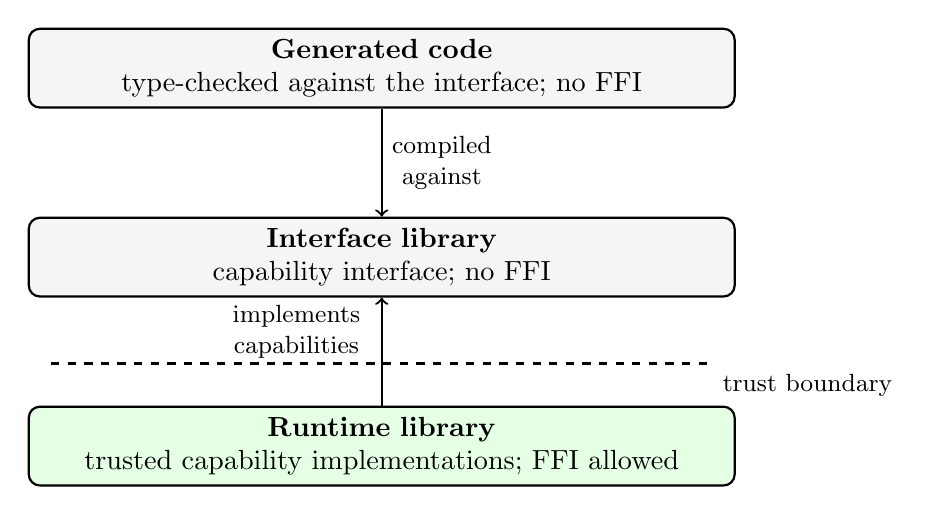
\begin{tikzpicture}[
  box/.style={draw, rounded corners, thick, align=center,
              text width=0.72\linewidth, minimum height=1.0cm},
  iface/.style={box, fill=gray!8},
  generated/.style={box, fill=gray!8},
  runtime/.style={box, fill=green!10},
  arrow/.style={->, thick},
  note/.style={font=\small, align=center}
]
  \node[generated] (ai) at (0,2.4)
    {\textbf{Generated code}\\type-checked against the interface; no FFI};
  \node[iface] (iface) at (0,0)
    {\textbf{Interface library}\\capability interface; no FFI};
  \node[runtime] (runtime) at (0,-2.4)
    {\textbf{Runtime library}\\trusted capability implementations; FFI allowed};

  \draw[dashed, thick] (-4.2,-1.35) -- (4.2,-1.35)
    node[note, below right]{trust boundary};
  \draw[arrow] (ai) -- node[note, right]{compiled\\against} (iface);
  \draw[arrow] (runtime) -- (iface);
  \node[note, left] at (-0.15,-0.95) {implements\\capabilities};
\end{tikzpicture}
\caption{Jo framework split for confining generated code. %
Only the runtime library below the trust boundary needs to be trusted.}
\label{fig:jo-framework-split}
\end{figure}

\autoref{fig:jo-framework-split} is the operational boundary. %
The interface library is the contract between the two sides. %
Generated code is not compiled against the runtime library, so it cannot name
its FFI-backed operations. %
Instead, generated code is compiled against the interface library, while the
trusted runtime library implements that interface and supplies concrete
capability values after generated code has been checked. %

In this example, the only input capability is \texttt{GetOrders}, a function
that returns orders for the current user, and the only output capability is
\texttt{IO.stdout}. %
The generated entry point must declare that it receives exactly those
capabilities. %

\begin{lstlisting}[style=pseudo]
param GetOrders: Int => List[Order]  // lastDays -> orders

defer def aiMain(): Unit receives GetOrders, IO.stdout
\end{lstlisting}

The framework constructs the actual capability values. %
It may internally use broad authority such as a database connection, the current
user identity, and a mutable output buffer. %
Those values remain in trusted code. %
The value given to generated code is an attenuated function that already
incorporates the user restriction. %

\begin{lstlisting}[style=pseudo]
def frameworkMain() =
  val db = connect("orders.db")
  val userId = currentUser()
  val restricted = (days: Int) => db.ordersFor(userId, days)

  val output: mutable.List[String] = []
  val buffer = (s: String) => output += s

  allow none in
    with GetOrders = restricted, IO.stdout = buffer in aiMain()
\end{lstlisting}

The generated program is checked against the interface it is allowed to use. %
It can read recent orders and write a summary, but it has no name for the
database, filesystem, network, or broader tool environment. %

\begin{lstlisting}[style=pseudo]
def aiMain(): Unit receives GetOrders, IO.stdout =
  val orders = GetOrders(30)
  summarize(orders)
\end{lstlisting}

\subsection{Why This Confines Authority}

The important point is where authority lives. %
The framework may possess broad authority, but it does not pass that authority
to generated code. %
Instead, it derives a narrower capability, \texttt{restricted}, and binds that
value as \texttt{GetOrders}. %
This is authority attenuation: the generated code can ask for orders, but only
through a function that has already fixed the user scope. %

\texttt{allow none} is also significant. %
It says that the body being run may not rely on ambient or already-in-scope
capabilities beyond those explicitly provided by the nested \texttt{with}. %
If generated code, or code reachable from it, requires some additional
capability, the compiler rejects the program. %
This gives the framework a static check that all direct and transitive
capability requirements have been mediated. %

This is the practical role of the captured-versus-caller-provided distinction in
the calculus. %
Trusted closures may capture broad internal state in order to build narrow
interfaces, but generated code receives only the caller-provided capabilities
listed in its signature and supplied at the call site. %
Captured authority is used to implement attenuation; caller-provided authority
is used to preserve control over invocation. %

The result is a design in which generated code can be useful without being
trusted with the whole runtime. %
It receives exactly the capabilities named by its interface, and the type system
checks that no additional capability is used. %

% related.tex - Related Work

\section{Related Work}
\label{sec:related}

The most relevant prior work falls into several groups. %

\subsection{Capability Disciplines Without Static Tracking}

Capability systems from Dennis and Van Horn onward \cite{dennis-vanhorn}
established the core authority model: capabilities are explicit,
unforgeable references to authority. %
Miller's object-capability account
\cite{miller-robust,miller-paradigm} and languages such as E \cite{e-lang},
Joe-E \cite{joe-e}, and Newspeak \cite{newspeak} demonstrate that this
discipline scales to realistic programming languages. %

What these systems give is a strong semantic and engineering story about
authority flow. %
What they generally do not give is a small static account of
which capabilities a term may use, nor a compact proof-oriented model of
fine-grained call-site capability provision. %

\subsection{Capability-Based Module Systems}

Wyvern is a closely related language-based security design. %
Melicher \etal{} \cite{melicher-wyvern} propose a capability-based module
system for authority control, and Fish \etal{} \cite{fish-wyvern-io} present
a case study building an I/O library for Wyvern. %
\lambdaCap{} shares the goal that I/O authority should be represented by
capabilities rather than ambient effects, but studies a smaller formal core in
which capability access is reflected directly in term typing and call-site
capability provision. %

\subsection{Static Requirement Tracking}

Lucassen and Gifford \cite{lucassen-gifford} and Talpin and Jouvelot
\cite{talpin-jouvelot} introduced influential frameworks for tracking
program requirements in types. %
 \lambdaCap{} follows that general direction,
but applies it specifically to capability access. %

The key difference is not merely that \lambdaCap{} tracks capabilities. %
It is
that it tracks them in a setting where some capabilities remain under
call-site control rather than being uniformly captured or manually threaded. %
In that sense, the model is also close in spirit to coeffects: it describes
what a computation requires from its context \cite{petricek-coeffects}. %

\subsection{Verified Capability Reasoning}

Swasey \etal{} \cite{swasey-caps} verify object-capability patterns in a
richer language using logical relations. %
Their work is closer in proof style
than in modeling goal: they verify specific patterns in a realistic setting,
whereas \lambdaCap{} isolates a minimal core calculus with global capability
soundness. %

Devriese and Piessens \cite{devriese-effect} show, in a different security
setting, that static reasoning can establish strong semantic guarantees. %
That
result is not about capabilities, but it supports the general thesis that
small static models can carry real security meaning. %

% explicitness.tex - Explicit capability specifications

\section{Should Capabilities Be Explicit?}
\label{sec:explicit-capabilities}

A central design question is how visible capabilities should be. %
One philosophy is that capabilities should remain visible in the program
structure, since visible authority supports review, audits, and a clear
security story. %
In private communication, the security expert Matt Rice has raised the concern
that hiding capability propagation can make it harder for reviewers to see
where authority flows. %

\lambdaCC{} leaves this choice to language and library designers. %
Because capabilities are statically tracked, a language can make capability
requirements explicit where that visibility matters, while still avoiding
manual propagation through every intermediate function. %
For example, a language may require public functions to have explicit capability
specifications. %
Such usability concerns are up to language designers' discretion. %
We believe it is good practice to make capability requirements explicit at
module boundaries. %
Within a module, contextual binding can reduce repetitive plumbing without
turning capabilities into ambient authority. %

% conclusion.tex - Conclusion

\section{Conclusion}
\label{sec:conclusion}

\lambdaCap{} is a small calculus aimed at three gaps in prior capability
work: the lack of a compact static account of capability use, the lack of a
clean formal model for fine-grained capability propagation through
higher-order code, and the lack of a corresponding foundation for simulation
and testing with explicit capability values. %

The model addresses these gaps with contextual capabilities: capabilities
that are tracked statically, yet may still be supplied by the calling context
rather than captured unconditionally. %
This makes it possible to reason about
two important patterns at once:
\begin{itemize}[nosep]
\item packaging attenuated authority into narrow interfaces, and
\item preserving caller control over invocation-time capabilities such as
  output channels or tool bindings. %
\end{itemize}

The soundness theorem shows that capability annotations are sound with
respect to evaluation. %
If the type system says a term uses no capabilities,
then evaluation succeeds with no capabilities provided. %
More generally, the
model supports rigorous reasoning about authority restriction, capability
containment, and higher-order confinement. %

The result is a verified semantic core for statically checked contextual
capabilities, especially relevant when executing untrusted or LLM-generated
code. %
Its main purpose is to guide the design of new secure programming
languages that make capability use explicit, statically checkable, and
controlled by program context. %

Resource bounds and covert channels are not addressed by this core calculus;
they must be handled by other means, such as runtime resource enforcement and
side-channel controls. %


\section*{Acknowledgments}

The authors thank Doctor Cl\'ement Blaudeau for discussions about the calculus. %

% Bibliography
\bibliographystyle{plain}
\begin{thebibliography}{99}

\bibitem{dennis-vanhorn}
J.~B. Dennis and E.~C. Van~Horn. %
\newblock Programming semantics for multiprogrammed computations. %
\newblock {\em Communications of the ACM}, 9(3):143--155, 1966. %

\bibitem{miller-robust}
M.~S. Miller. %
\newblock {\em Robust Composition: Towards a Unified Approach to Access Control
  and Concurrency Control}. %
\newblock PhD thesis, Johns Hopkins University, 2006. %

\bibitem{miller-paradigm}
M.~S. Miller, K.-P. Yee, and J.~Shapiro. %
\newblock Capability myths demolished. %
\newblock Technical Report SRL2003-02, Johns Hopkins University, 2003. %

\bibitem{e-lang}
M.~S. Miller, E.~D. Tribble, and J.~Shapiro. %
\newblock Concurrency among strangers: Programming in {E} as plan coordination. %
\newblock In {\em Symposium on Trustworthy Global Computing}, pages 195--229. %
  Springer, 2005. %

\bibitem{joe-e}
A.~Mettler, D.~Wagner, and T.~Close. %
\newblock Joe-{E}: A security-oriented subset of {J}ava. %
\newblock In {\em Network and Distributed System Security Symposium (NDSS)},
  2010. %

\bibitem{newspeak}
G.~Bracha and D.~Ungar. %
\newblock Mirrors: Design principles for meta-level facilities of
  object-oriented programming languages. %
\newblock In {\em OOPSLA}, pages 331--344, 2004. %

\bibitem{melicher-wyvern}
D.~Melicher, Y.~Shi, A.~Potanin, and J.~Aldrich. %
\newblock A capability-based module system for authority control. %
\newblock In {\em European Conference on Object-Oriented Programming (ECOOP)},
  2017. %

\bibitem{fish-wyvern-io}
J.~Fish, D.~Melicher, and J.~Aldrich. %
\newblock A case study in language-based security: Building an {I/O} library
  for {Wyvern}. %
\newblock In {\em ACM SIGPLAN International Symposium on New Ideas, New
  Paradigms, and Reflections on Programming and Software (Onward!)}, 2020. %

\bibitem{saltzer-schroeder}
J.~H. Saltzer and M.~D. Schroeder. %
\newblock The protection of information in computer systems. %
\newblock {\em Proceedings of the IEEE}, 63(9):1278--1308, 1975. %

\bibitem{hardy-confused}
N.~Hardy. %
\newblock The confused deputy: (or why capabilities might have been invented). %
\newblock {\em ACM SIGOPS Operating Systems Review}, 22(4):36--38, 1988. %

\bibitem{liu-jo-design}
F.~Liu, C.~Blaudeau, and O.~Lhot\'ak. %
\newblock A parametric design of globals and capabilities. %
\newblock 2026. %

\bibitem{devriese-effect}
D.~Devriese and F.~Piessens. %
\newblock Noninterference through secure multi-execution. %
\newblock In {\em IEEE Symposium on Security and Privacy}, pages 109--124, 2010. %

\bibitem{swasey-caps}
D.~Swasey, D.~Garg, and D.~Dreyer. %
\newblock Robust and compositional verification of object capability patterns. %
\newblock {\em Proceedings of the ACM on Programming Languages}, 1(OOPSLA):1--26,
  2017. %

\bibitem{lucassen-gifford}
J.~M. Lucassen and D.~K. Gifford. %
\newblock Polymorphic effect systems. %
\newblock In {\em Proceedings of the 15th ACM SIGPLAN-SIGACT symposium on
  Principles of programming languages}, pages 47--57, 1988. %

\bibitem{talpin-jouvelot}
J.-P. Talpin and P.~Jouvelot. %
\newblock Polymorphic type, region and effect inference. %
\newblock {\em Journal of Functional Programming}, 2(3):245--271, 1992. %

\bibitem{petricek-coeffects}
T.~Petricek, D.~Orchard, and A.~Mycroft. %
\newblock Coeffects: A calculus of context-dependent computation. %
\newblock In {\em Proceedings of the 19th ACM SIGPLAN International Conference
  on Functional Programming}, pages 123--135, 2014. %

\bibitem{pierce-tapl}
B.~C. Pierce. %
\newblock {\em Types and Programming Languages}. %
\newblock MIT Press, 2002. %

\bibitem{pierce-atapl}
B.~C. Pierce, editor. %
\newblock {\em Advanced Topics in Types and Programming Languages}. %
\newblock MIT Press, 2005. %

\end{thebibliography}

\end{document}
